% これは1カラムで表示する図
\begin{figure}[t]
  \begin{center}
    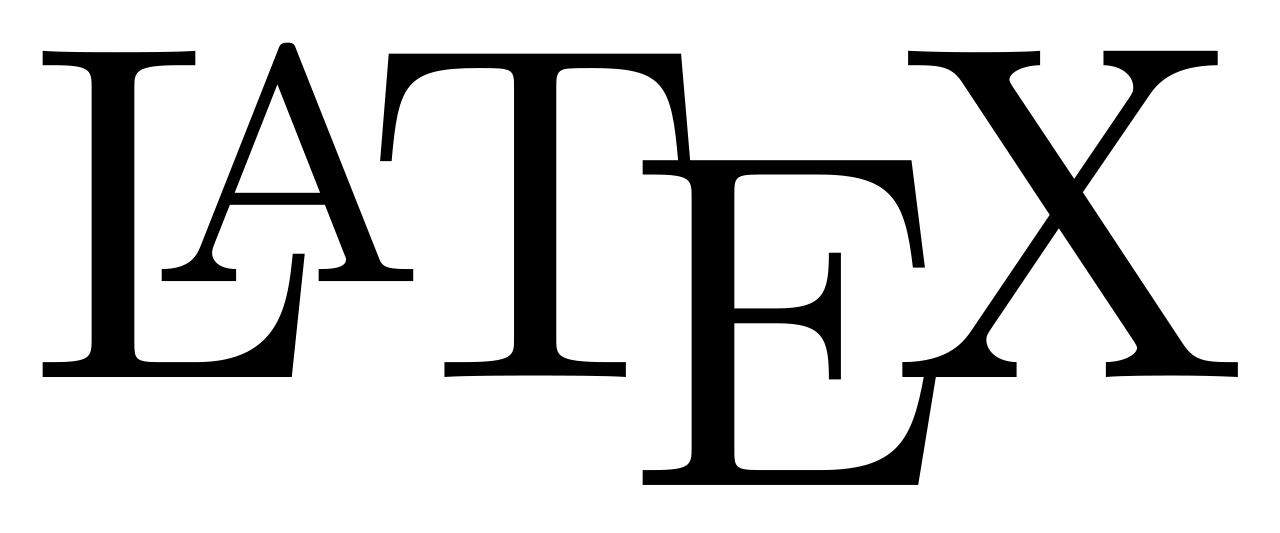
\includegraphics[width=8.5cm]{figs/latex_logo.png}
    \caption{latex logo half}
    \label{fig:latex_logo_half}
  \end{center}
\end{figure}

% これは2カラムで表示する図
\begin{figure*}[t]
\centering
    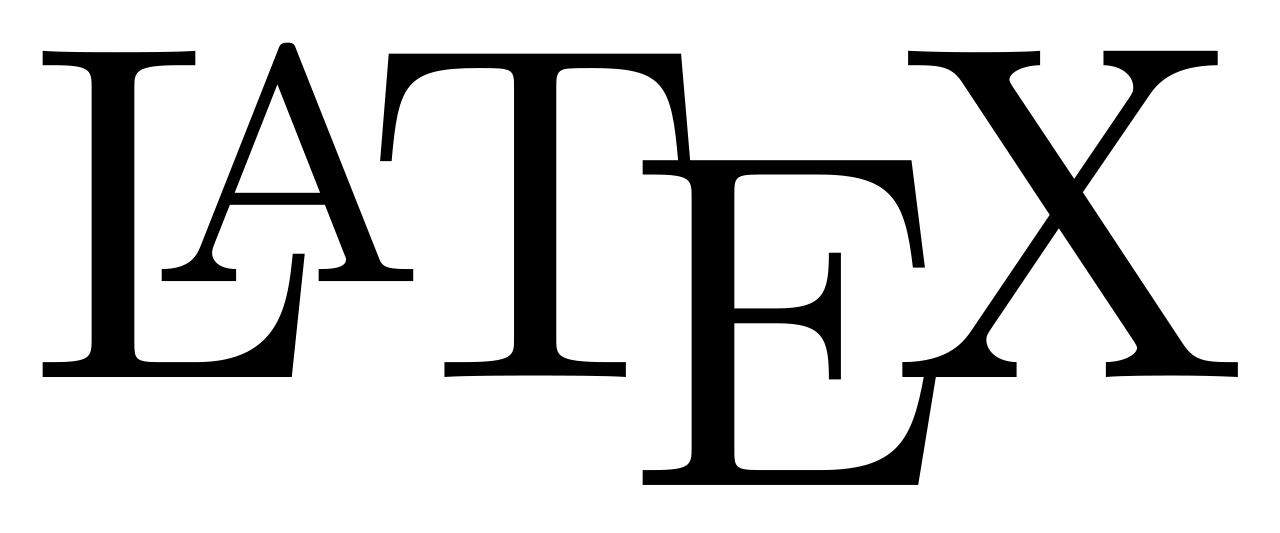
\includegraphics[width=\textwidth]{./figs/latex_logo.png}
    \caption{latex logo}
    \label{fig:latex_logo}
\end{figure*}

% テーブル
\begin{table}[t]
    \centering
\caption{定量評価結果}
\label{tab:quantitative_eval}
\begin{tabular}{ccccc}
    \toprule
& 手法A & 手法B & Ours \\
    \midrule
指標A & 123.5 & 126.9 & {\bf 142.1} \\
指標B & 0.887 & 0.910 & {\bf 0.956} \\
\bottomrule
\end{tabular}
\end{table}

\section{図と表と式}
大きく画像を表示したい時は\figref{fig:latex_logo}.
2カラムの時に小さく画像を表示したい時は\figref{fig:latex_logo_half}.
表は\tabref{tab:quantitative_eval}.
式は以下のように記述すれば良い.
%
% テーブル
\begin{equation}
\label{eq:gauss}
f(x | \mu, \sigma^2) = \frac{1}{\sqrt{2 \pi \sigma^2}} e^{-\frac{(x - u)^2}{2 \sigma^2}}
\end{equation}
\equref{eq:gauss}で引用可能.
%
参考文献の引用はこんな感じ\cite{goodfellow2014generative}.